\section{Computations for small orders}
\label{sec:computations}

All counts below were computed in exact integer arithmetic; the methods are described in \Cref{sec:appendix}, and every number is produced by a script in the ancillary directory \texttt{anc/}.

\subsection{The low-order class for \texorpdfstring{$n=4$}{n=4}}
\label{sec:lowmode_n4}

Let $L_n$ be the set of arrangements with $\Elow=0$, i.e.\ $\Cov(X,Z)=\Cov(Y,Z)=0$ and both diagonal sums equal to $M(n)$.
With cells indexed by $(i,j)$, these are the conditions $U_1=U_2=\frac{n-1}2\cdot\frac{N(N+1)}2$ and $U_3=U_4=M(n)$ on the sums
$U_1=\sum_{i,j}j\,s_{ij}$, $U_2=\sum_{i,j}i\,s_{ij}$, $U_3=\sum_is_{ii}$, $U_4=\sum_is_{i,n-1-i}$, which are additive over cells.

\begin{proposition}[The size of $L_4$]
\label{prop:L4}
$|L_3|=8$ (the magic squares), and
\[
|L_4|=14{,}639{,}440=8\times1{,}829{,}930,
\]
of which $7{,}040$ are magic squares.
The class $\{\Cov(X,Z)=\Cov(Y,Z)=0\}$ has $6{,}697{,}177{,}424$ members for $n=4$, and the class with both diagonal sums equal to $34$ has $49{,}932{,}288{,}000$.
\end{proposition}

\begin{proof}[Computation]
A meet-in-the-middle enumeration over $(U_1,\dots,U_4)$, splitting the grid into the top two and bottom two rows (\Cref{sec:appendix}); the matching pairs were expanded to obtain the breakdown of \Cref{tab:L4}.
The same program reproduces the brute-force counts for $n=3$ ($8$, $760$, $4224$, and $72$ semi-magic squares) and, with the $2n$ line sums in place of $U_1,U_2$, the $7{,}040$ magic and $549{,}504$ semi-magic squares of order $4$.
The diagonal-only count also follows from a direct count: there are $2150$ ordered pairs of disjoint $4$-subsets of $\{1,\dots,16\}$ with sum $34$, and $2150\cdot(4!)^2\cdot8!=49{,}932{,}288{,}000$.
\end{proof}

Since $D_4$ acts freely on the set of all arrangements (entries are distinct) and preserves $L_4$, $L_4$ consists of $1{,}829{,}930$ orbits of size $8$.

\begin{table}[htbp]
\centering
\small
\begin{tabular}{lrrrr}
\toprule
 & \multicolumn{4}{c}{columns with sum 34} \\
\cmidrule(lr){2-5}
rows with sum 34 & 0 & 1 & 4 & total \\
\midrule
0 & 9\,637\,312 & 2\,172\,824 & 100\,728 & 11\,910\,864 \\
1 & 2\,172\,824 & 429\,312 & 9\,336 & 2\,611\,472 \\
4 & 100\,728 & 9\,336 & \textbf{7\,040} (magic) & 117\,104 \\
\midrule
total & 11\,910\,864 & 2\,611\,472 & 117\,104 & 14\,639\,440 \\
\bottomrule
\end{tabular}
\caption{The members of $L_4$ by the number of rows and of columns with sum $M(4)=34$; the table is symmetric under transposition.}
\label{tab:L4}
\end{table}

Exactly two or three rows with sum $34$ are impossible in $L_4$: the row deviations $e_i$ satisfy $\sum_ie_i=0$ and $\sum_iie_i=0$, which cannot hold with exactly one or two nonzero $e_i$; the same holds for columns.
Thus $7040/14{,}639{,}440\approx0.048\%$ of $L_4$ is magic, and $9{,}637{,}312$ members ($66\%$) have no row or column with sum $34$, among them the arrangement of \Cref{rem:four_term_insufficient}.

\paragraph{A local-limit estimate.}
Under a uniformly random arrangement the vector $(U_1,\dots,U_4)$ has mean equal to the target vector and covariance matrix $\Sigma_U$ given by \eqref{eq:ww_identity}: $U_1,U_2$ are uncorrelated with each other and with the diagonal sums, which have correlation $-1/(n-1)$ for even $n$ and $0$ for odd $n$.
The single transpositions change $(U_1,\dots,U_4)$ by vectors whose $\Z$-span is $\Z^4$ (Smith normal form, $n\le8$).
A Gaussian local limit would therefore give $|L_n|\approx N!\,(2\pi)^{-2}\det(\Sigma_U)^{-1/2}$.
This estimate is $13.6$ for $n=3$ ($|L_3|=8$) and $1.82\times10^{7}$ for $n=4$, so $|L_4|$ is $0.80$ times the estimate; for the two-condition classes the ratios at $n=3,4$ are $0.59,0.91$ (first moments) and $1.10,0.96$ (diagonals).
For $n=5,6$ Monte Carlo ($10^{10}$ and $2\times10^{10}$ samples, $328$ and $62$ members of $L_n$) gives $|L_5|\approx5.1\times10^{17}$ ($\pm6\%$) and $|L_6|\approx1.2\times10^{33}$ ($\pm13\%$), ratios $0.76$ and $0.78$ to the estimate.
Since $\det(\Sigma_U)^{1/2}$ grows like $n^{13}$, one expects $|L_n|/N!$ to decay like $n^{-13}$, and the fraction of magic squares in $L_n$ to tend to $0$; local limit theorems for permutation statistics of this kind are studied in \cite{kuperberg2017probabilistic,eberhard2019additive}, and related counts of matrices with prescribed margins in \cite{canfield2010asymptotic}.

\subsection{Single swaps}
\label{sec:swap-gaps}

\begin{remark}[Single-swap formula]
\label{rem:swap}
Let $S^{ab}$ be obtained from $S$ by exchanging the entries of cells $a\ne b$, let $d=s_b-s_a$, let $\lambda(a,b)$ be the number of lines containing exactly one of $a,b$, and $u_S(c)=\sum_{L\ni c}\delta_L(S)$.
Expanding \eqref{eq:Efull_devs},
\[
N^{2}\bigl(\Efull(S^{ab})-\Efull(S)\bigr)=d^{2}\lambda(a,b)+2d\bigl(u_S(a)-u_S(b)\bigr),
\]
the incremental evaluation used in local search \cite{pinn1998number}.
Here $\lambda(a,b)=2[i\ne i']+2[j\ne j']+[\text{a diagonal separates }a,b]+[\text{the other diagonal separates }a,b]\in\{2,\dots,6\}$ for $a=(i,j)$, $b=(i',j')$.
For a magic square $S$, $N^2\Efull(S^{ab})=d^2\lambda(a,b)\ge2$, so no two magic squares differ by a transposition, and the values lie in the set $\{d^2\lambda:1\le d\le N-1,\ 2\le\lambda\le6\}$.
The smallest value $g_{\min}(S)=\min_{a\ne b}d^2\lambda(a,b)$ satisfies $2\le g_{\min}(S)\le6$: the value $2$ occurs if and only if two consecutive values lie in a common row or column and off both diagonals, and consecutive values give at most $6$.
\end{remark}

Over the $880\cdot\binom{16}2=105{,}600$ swaps of the $880$ magic squares of order $4$ up to $D_4$, the gap $d^2\lambda$ takes $70$ values from $2$ to $980$, and $g_{\min}(S)$ is $2$ for $432$ squares, $3$ for $420$ and $4$ for $28$ (\Cref{fig:swap_spectrum}); it is $3$ for the magic squares of order $3$.
For $n=3$, besides the eight magic squares, $\Efull$ has eight non-magic local minima with respect to swaps, all with $N^2\Efull=2$; $\Elow$ has $344$ local minima, of which $336$ are non-magic.
Steepest swap descent on $\Efull$ from a random arrangement reaches a magic square in $19.5\%$ of runs for $n=4$, $1.2\%$ for $n=5$ and $0.8\%$ for $n=6$ (\texttt{anc/algorithms.py}).

\begin{figure}[htbp]
\centering
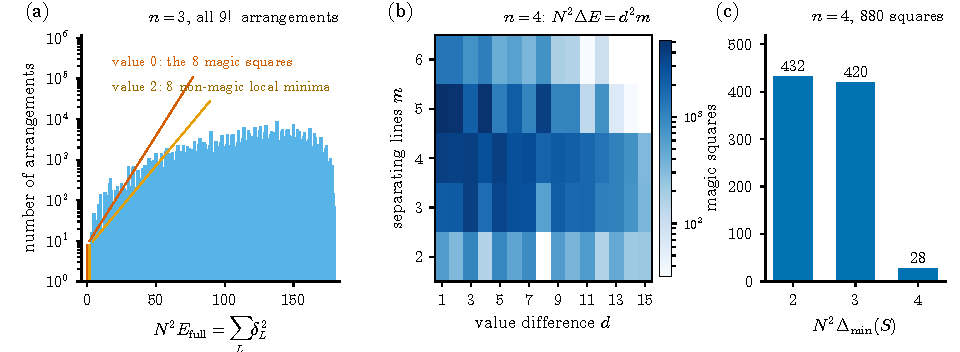
\includegraphics[width=\textwidth]{figures/fig_swap_spectrum.pdf}
\caption{Swap gaps. (a)~For $n=3$, the number of arrangements with each value of $N^2\Efull=\sum_L\delta_L^2$; the eight magic squares are at $0$ and the eight non-magic local minima at $2$. (b)~For $n=4$, the number of single swaps of the $880$ magic squares ($105{,}600$ in total) by value difference $d$ and number $\lambda$ of separating lines; the gap is $d^2\lambda$. (c)~The smallest gap $g_{\min}(S)$ over the $880$ squares.}
\label{fig:swap_spectrum}
\end{figure}
